% vim: ts=8 sts=8 sw=4 et tw=75
\chapter{小型语言}
\label{chap:little_languages}
\marginpar{131}

人们经常使用 awk 开发 ``小型语言'' 的翻译器 (``小型语言'' 指的特定于
某些应用领域的专用编程语言), 
开发翻译器的原因主要有三点. 首先, 它可以帮助你了解语言处理程序的工作流程.
本章的第一个例子是一个汇编程序, 虽然只有 20 来行, 但已经包含了汇编过程
的核心要素, 为了执行汇编程序, 我们还要开发一个解释程序. 汇编程序与
解释程序反映了早期阶段汇编语言与机器架构的关系. 其他例子还包括一个
后缀计算器, awk 子集的递归下降分析器.

第二个原因是在实际工作中, 为了实现一个专用的编程语言, 通常需要投入大
量的精力与财力, 不过在这之前, 我们有必要测试一下新语言的语法和语义. 
作为示例, 本章讨论了一个画图语言和一个参数设置语言, 后者用于设置排序命令
的参数.

最后一点是希望编程语言能够在实际的工作发挥作用, 就比如说本章所开发的
计算器.

语言处理程序围绕下面这个模型构造而成:
\begin{center}
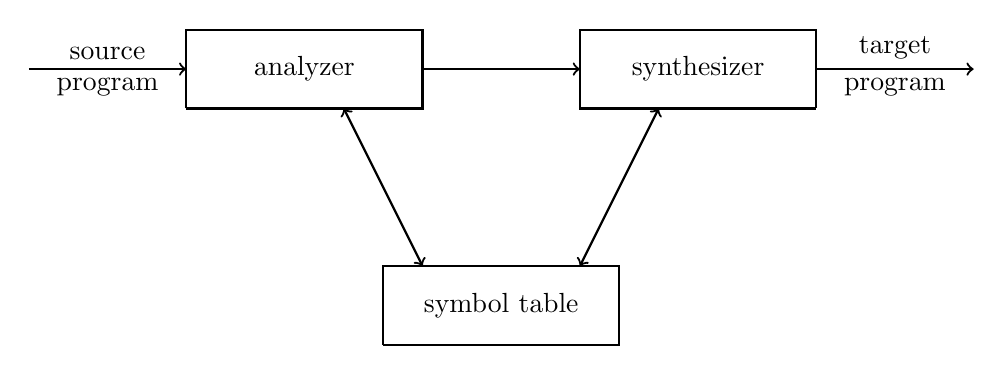
\begin{tikzpicture}
    \draw[thick]
        (-1.5, 0) -- (-1.5, 1.0) -- (1.5, 1.0) -- (1.5, 0) -- (-1.5, 0);
    \draw[thick]
        (-4.0, 3.0) -- (-4.0, 4.0) -- (-1.0, 4.0) -- (-1.0, 3.0) -- (-4.0,
        3.0);
    \draw[thick]
        (4.0, 3.0) -- (4.0, 4.0) -- (1.0, 4.0) -- (1.0, 3.0) -- (4.0, 3.0);
    
    \draw[thick,->]
        (-6.0, 3.5) -- (-4.0, 3.5);
    \draw[thick,->]
        (-1.0, 3.5) -- (1.0, 3.5);
    \draw[thick,->]
        (4.0, 3.5) -- (6.0, 3.5);
    \draw[thick,<->]
        (-2.0, 3.0) -- (-1.0, 1.0);
    \draw[thick,<->]
        (2.0, 3.0) -- (1.0, 1.0);

    \node[above] at (-5.0, 3.5) {source};
    \node[below] at (-5.0, 3.5) {program};
    \node at (-2.5, 3.5) {analyzer};
    \node at (2.5, 3.5) {synthesizer};
    \node[above] at (5.0, 3.5) {target};
    \node[below] at (5.0, 3.5) {program};
    \node at (0, 0.5) {symbol table};
\end{tikzpicture}
\end{center}

分析器 (analyzer) 系语言处理程序的前端, 它负责读取源程序 (source program)
并将其切分成 一个个词法单元, 词法
单元包括运算符, 操作数等. 分析器对源程序进行语法检查, 如果源程序含有语法
错误, 它就会打印一条错误消息. 最后, 分析器把源程序转换成某种中间形式,
并传递给后端 (合成器), 合成器 (synthesizer) 再根据中间形式生成目标程序
(target program). 合成器在生成
目标程序的过程中需要和符号表 (symbol table) 通信, 而符号表中的内容由分析
器收集而来.
虽然我们把语言的处理过程描述成多个界限分明的不同步骤, 但实际上, 这些界限
通常很模糊, 而且有些步骤有可能被合并成一个.
\marginpar{132}

利用 awk 为实验性语言构造处理程序非常方便, 这是因为它支持许多和语言翻译
相关的操作. 对源程序的分析可以通过字段分割与正则表达式来完成, 用关联数组
管理符号表, 用 \texttt{printf} 生成目标代码.

关于上面提到的几点, 我们将通过开发几个翻译器来进一步说明. 在保证足够说明
问题的前提下,  将尽量保持程序的简短, 而把润色与优化留到习题中.

\section{汇编程序与解释程序}
\label{subsec:an_assembler_and_interpreter}

我们的第一个例子是虚拟计算机的汇编程序, 虚拟计算机这个概念经常出现在
计算机体系 结构或系统编程的基础课程中. 虚拟计算机有一个累加器, 十条
指令, 按字编址且大小为 1000 字的内存, 我们假设内存的一个 ``字'' 可以
保存5个十进制数位, 如果某个字存放的是一条指令, 那么前两个数位表示操作
码, 最后三个数位表示内存地址. 所有的汇编语言指令在表
\ref{tbl:assembly_language_instructions} 中列出.
\begin{figure}[ht]
\captionsetup{type=table}
\caption{汇编语言指令集}
\label{tbl:assembly_language_instructions}
\begin{center}
    \begin{tabular}{c|l|l}
        \hline
        \hline
        操作码          & 指令    &
        \multicolumn{1}{c}{意义}  \\
        \hline
        \texttt{01}     & \texttt{get}  & 从输入读取一个数, 并存放到累
        加器中 \\
        \texttt{02}     & \texttt{put}  & 把累加器的值写到输出 \\
        \texttt{03}     & \texttt{ld M}  & 把地址为 \texttt{M} 的内存单元
        的值读取到累加器中 \\
        \texttt{04}     & \texttt{st M}  & 把累加器的值存放到地址为 
        \texttt{M} 的内存单元中 \\
        \texttt{05}     & \texttt{add M} & 把地址为 \texttt{M} 的内存单元 
        的值与累加器的值相加, 再把结果存放到累加器中 \\
        \texttt{06}     & \texttt{sub M} & 把地址为 \texttt{M} 的内存单元 
        的值与累加器的值相减, 再把结果存放到累加器中 \\
        \texttt{07}     & \texttt{jpos M} & 如果累加器的值为正, 则跳转到
        内存地址 \texttt{M} \\
        \texttt{08}     & \texttt{jz M} & 如果累加器的值为零, 则跳转到 
        内存地址 \texttt{M}     \\
        \texttt{09}     & \texttt{j M}  & 跳转到内存地址 \texttt{M} \\
        \texttt{10}     & \texttt{halt} & 停止执行 \\
                        & \texttt{const C} & 伪操作符, 用于定义一个常量
                        \texttt{C} \\
        \hline
    \end{tabular}
\end{center}
\end{figure}

汇编语言程序由语句序列组成, 每一条语句都包括三个部分: 标号, 操作符, 
操作数, 任意一个部分都可以省略, 标号如果存在, 则必须是所在行的第一个
字段. 程序可以包含 awk 形式的注释. 这里有一个简单的汇编语言程序, 它
的功能是输出多个整数的和, 0 表示输入结束.
\marginpar{133}
\begin{file}
    # print sum of input numbers (terminated by zero)

         ld    zero   # initialize sum to zero
         st    sum
    loop get          # read a number
         jz    done   # no more input if number is zero
         add   sum    # add in accumulated sum
         st    sum    # store new value back in sum
         j     loop   # go back and read another number

    done ld    sum    # print sum
         put
         halt

    zero const 0
    sum  const
\end{file}

对应的目标程序由整数序列组成, 这些整数其实就是程序的机器码形式, 当目标
程序运行时, CPU 从内存中读取指令, 译码并执行. 上面程序的机器码是:
\begin{file}
     0: 03010           ld      zero    # initialize sum to zero
     1: 04011           st      sum
     2: 01000      loop get             # read a number
     3: 08007           jz      done    # no more input if number is zero
     4: 05011           add     sum     # add in accumulated sum
     5: 04011           st      sum     # store new value back in sum
     6: 09002           j       loop    # go back and read another number
     7: 03011      done ld      sum     # print sum
     8: 02000           put
     9: 10000           halt
    10: 00000      zero const 0
    11: 00000      sum  const
\end{file}
第一个字段是内存地址, 第二个字段是编码后的指令. 内存地址 0 存放的是汇编
语言程序的第一条指令: \texttt{ld zero}.

汇编程序对源程序进行汇编时需要遍历两次. 第一次遍历利用字段分割操作对源
程序进行词法与语法检查: 读取汇编语言源程序, 忽略注释, 为每一个标号分配
内存地址, 把操作符与操作数的中间表示形式写到一个临时文件中. 第二次遍历
读取临时文件, 根据第一次遍历时计算的结果, 把符号化的操作数转换成内存地
址, 对操作符与操作数进行编码, 把最终的机器语言程序保存到数组 \texttt{mem}
中.

我们将会开发一个解释器来完成另一半的工作, 解释器可以用来模拟计算机执行
机器语言程序时所表现出的行为. 解释器循环地从 \texttt{mem} 中读取指令,
把指令译码成操作符与操作数, 再模拟指令的执行. 变量 \texttt{pc} 用来模拟
程序计数器 (program counter).
\marginpar{134}
\begin{awkcode}
    # asm - assembler and interpreter for simple computer
    #   usage: awk -f asm program-file data-files...

    BEGIN {
        srcfile = ARGV[1]
        ARGV[1] = ""  # remaining files are data
        tempfile = "asm.temp"
        n = split("const get put ld st add sub jpos jz j halt", x)
        for (i = 1; i <= n; i++)   # create table of op codes
            op[x[i]] = i-1

    # ASSEMBLER PASS 1
        FS = "[ \t]+"
        while (getline <srcfile > 0) {
            sub(/#.*/, "")         # strip comments
            symtab[$1] = nextmem   # remember label location
            if ($2 != "") {        # save op, addr if present
                print $2 "\t" $3 >tempfile
                nextmem++
            }
        }
        close(tempfile)

    # ASSEMBLER PASS 2
        nextmem = 0
        while (getline <tempfile > 0) {
            if ($2 !~ /^[0-9]*$/)  # if symbolic addr,
                $2 = symtab[$2]    # replace by numeric value
            mem[nextmem++] = 1000 * op[$1] + $2  # pack into word
        }

    # INTERPRETER
        for (pc = 0; pc >= 0; ) {
            addr = mem[pc] % 1000
            code = int(mem[pc++] / 1000)
            if      (code == op["get"])  { getline acc }
            else if (code == op["put"])  { print acc }
            else if (code == op["st"])   { mem[addr] = acc }
            else if (code == op["ld"])   { acc  = mem[addr] }
            else if (code == op["add"])  { acc += mem[addr] }
            else if (code == op["sub"])  { acc -= mem[addr] }
            else if (code == op["jpos"]) { if (acc >  0) pc = addr }
            else if (code == op["jz"])   { if (acc == 0) pc = addr }
            else if (code == op["j"])    { pc = addr }
            else if (code == op["halt"]) { pc = -1 }
            else                         { pc = -1 }
        }
    }
\end{awkcode}

数组 \texttt{symtab} 记录标号的内存地址, 如果当前输入行没有标号, 那么内存
地址赋值给 \texttt{symtab[""]}.

标号是汇编语句的第一个字段, 操作符前面有一个空格符. 第一次遍历前, 把
\marginpar{135}
\texttt{FS} 设置成 \verb'[ \t]+', 于是字段分隔符变成由多个空格符和制表
符组成的序列. 比较特殊的是, 前导空格也被当作字段分隔符, 所以 \verb'$1'
总是标号, 而 \verb'$2' 总是操作符.

因为伪操作符 \texttt{const} 的操作码是 0, 所以在第二次遍历时, 语句
\begin{awkcode}
    mem[nextmem++] = 1000 * op[$1] + $2  # pack into word
\end{awkcode}
可以同时用来存放常数与指令.

\begin{exercise}
    修改 \texttt{asm}, 打印程序与内存的内容, 就像上面显示的那样.
\end{exercise}

\begin{exercise}
    增强解释器的功能, 打印指令的执行轨迹.
\end{exercise}

\begin{exercise}
    适当扩大汇编语言的规模, 比如添加错误处理代码与其他条件判断指令. 为了 
    方便用户使用, 你会怎么处理立即数, 比如 \texttt{add = 1} (如果 
    不支持立即数, 就必须要求用户自己创建一个名为 \texttt{one} 的
    内存单元)?
\end{exercise}

\begin{exercise}
    写一个反汇编程序, 把内存中的内容转换成对应的汇编语言.
\end{exercise}

\begin{exercise}
    查看一台真实的机器 (比如 Apple-II 和 Commodore 的 6502 芯片, 或
    IBM PC 及其兼容机的 8086 芯片族), 尝试为它的汇编语言子集写
    一个汇编程序.
\end{exercise}

\section{画图语言}
\label{sec:a_language_for_drawing_graphs}

利用字段分割操作, 很容易就可以对我们自己定义的汇编语言作词法和语法分析,
这种简易性对一些高级语言来说同样成立. 我们的下一个例子是 \texttt{graph} 
的语言处理程序, \texttt{graph} 是一种用来画数据坐标图的原型语言. 输入
是一张图的规范说明, 规范说明的每一行都表示一个数据点, 或坐标轴的标签
信息. 数据点由一对 \textit{x}-\textit{y} 表示, 如果只有一个 \textit{y},
则 \textit{x} 是从 1 开始的递增序列, 即 1, 2, 3, ..., 
An optional nonnumeric plotting character can follow either form of data
value\footnote{TODO}. 标签信息由一个关键词和多个参数值组成:
\begin{pattern}
\indent\texttt{label}\ \textit{caption} \par
\indent\texttt{range}\ \textit{xmin}\ \textit{ymin}\ \textit{xmax}\
    \textit{ymax} \par 
\indent\texttt{left ticks}\ \ \textit{t}$_1$\ \textit{t}$_2$ ... \par 
\indent\texttt{bottom ticks}\ \ \textit{t}$_1$\ \textit{t}$_2$ ... \par 
\indent\texttt{height}\ \textit{number}\par
\indent\texttt{width}\ \textit{number}\par
\end{pattern}
这些行的出现顺序是任意的, 任意一行都可以省略, 也不需要指定数据的值的
范围.

处理程序按比例调整数据点的大小, 并生成绘图命令. 为了使讨论更加具体,
我们把它们打印到 $24 \times 80$ 的字符数组中, 但是, 如果是为某些
图像设备生成绘图命令, 实现起来其实也很容易. 例如, 输入数据:
\marginpar{136}
\begin{file}
    label Annual Traffic Deaths, USA, 1925-1984
    range 1920 5000 1990 60000
    left ticks 10000 30000 50000
    bottom ticks 1930 1940 1950 1960 1970 1980

    1925 21800
    1930 31050
    1935 36369
    ...
    1981 51500
    1982 46000
    1983 44600
    1984 46200
\end{file}
的输出是\footnote{输入数据是我瞎编的, 所以生成的坐标图与英文原版
不太一致 --- 译者注}:
{\small
\begin{file}
      |------------------------------------------------------------------------|
      |                                                                        |
      |                                                                        |
      |                                                     **    *   *        |
50000 -                                                    *   * *   *         |
      |                                                   *            * *     |
      |                                                         *       *      |
      |                                                ***    *     *          |
      |                                *     *     ****                        |
      |               *                 *  *   *                               |
      |                          **  **  *       **                            |
30000 -         *          *       **       * * *                              |
      |                         *                                              |
      |                                                                        |
      |                                                                        |
      |    *                                                                   |
      |                                                                        |
      |                                                                        |
      |                                                                        |
10000 -                                                                        |
      |                                                                        |
      |---------|----------|---------|----------|---------|----------|---------|
               1930       1940      1950       1960      1970       1980        
                        Annual Traffic Deaths, USA, 1925-1984                   
\end{file}
}

\texttt{graph} 的处理程序分为两个阶段. 主循环读取并解析图的规范说明, 
使用模式辨认不同类型的语句. 图的中间表示形式存放在若干个数组与变量中,
如果必要的话, \texttt{END} 据此计算值的范围, 然后开始绘制边框, 刻度,
标签和数据点. 输出操作被分散在若干个函数中, 这样的话, 即使以后要为
特定的设备对代码进行修改, 也可以把修改局限在小范围内.

到目前为止, 这是我们看过的最长的 awk 程序, 大约有 100 行, 其实它是本书
第二长的程序. 不过不要担心, 程序把一个大任务分成若干个小步骤来完成, 
所以每个部分都很简短.
\marginpar{137}
\begin{awkcode}
    # graph - processor for a graph-drawing language
    #   input:  data and specification of a graph
    #   output: data plotted in specified area

    BEGIN {                # set frame dimensions...
        ht = 24; wid = 80  # height and width
        ox = 6; oy = 2     # offset for x and y axes
        number = "^[-+]?([0-9]+[.]?[0-9]*|[.][0-9]+)" \
                                "([eE][-+]?[0-9]+)?$"
    }
    $1 == "label" {                       # for bottom
        sub(/^ *label */, "")
        botlab = $0
        next
    }
    $1 == "bottom" && $2 == "ticks" {     # ticks for x-axis
        for (i = 3; i <= NF; i++) bticks[++nb] = $i
        next
    }
    $1 == "left" && $2 == "ticks" {       # ticks for y-axis
        for (i = 3; i <= NF; i++) lticks[++nl] = $i
        next
    }
    $1 == "range" {                       # xmin ymin xmax ymax
        xmin = $2; ymin = $3; xmax = $4; ymax = $5
        next
    }
    $1 == "height" { ht = $2; next }
    $1 == "width"  { wid = $2; next }
    $1 ~ number && $2 ~ number {          # pair of numbers
        nd++    # count number of data points
        x[nd] = $1; y[nd] = $2
        ch[nd] = $3    # optional plotting character
        next
    }
    $1 ~ number && $2 !~ number {         # single number
        nd++    # count number of data points
        x[nd] = nd; y[nd] = $1; ch[nd] = $2
        next
    }
    END {    # draw graph
        if (xmin == "") {         # no range was given
            xmin = xmax = x[1]    # so compute it
            ymin = ymax = y[1]
            for (i = 2; i <= nd; i++) {
                if (x[i] < xmin) xmin = x[i]
                if (x[i] > xmax) xmax = x[i]
                if (y[i] < ymin) ymin = y[i]
                if (y[i] > ymax) ymax = y[i]
            }
        }
        frame(); ticks(); label(); data(); draw()
    }
\end{awkcode}
\marginpar{138}
\begin{awkcode}
    function frame() {        # create frame for graph
        for (i = ox; i < wid; i++) plot(i, oy, "-")     # bottom
        for (i = ox; i < wid; i++) plot(i, ht-1, "-")   # top
        for (i = oy; i < ht; i++) plot(ox, i, "|")      # left
        for (i = oy; i < ht; i++) plot(wid-1, i, "|")   # right
    }
    function ticks(    i) {   # create tick marks for both axes
        for (i = 1; i <= nb; i++) {
            plot(xscale(bticks[i]), oy, "|")
            splot(xscale(bticks[i])-1, 1, bticks[i])
        }
        for (i = 1; i <= nl; i++) {
            plot(ox, yscale(lticks[i]), "-")
            splot(0, yscale(lticks[i]), lticks[i])
        }
    }
    function label() {        # center label under x-axis
        splot(int((wid + ox - length(botlab))/2), 0, botlab)
    }
    function data(    i) {    # create data points
        for (i = 1; i <= nd; i++)
            plot(xscale(x[i]),yscale(y[i]),ch[i]=="" ? "*" : ch[i])
    }
    function draw(    i, j) { # print graph from array
        for (i = ht-1; i >= 0; i--) {
            for (j = 0; j < wid; j++)
                printf((j,i) in array ? array[j,i] : " ")
            printf("\n")
        }
    }
    function xscale(x) {      # scale x-value
        return int((x-xmin)/(xmax-xmin) * (wid-1-ox) + ox + 0.5)
    }
    function yscale(y) {      # scale y-value
        return int((y-ymin)/(ymax-ymin) * (ht-1-oy) + oy + 0.5)
    }
    function plot(x, y, c) {  # put character c in array
        array[x,y] = c
    }
    function splot(x, y, s,    i, n) { # put string s in array
        n = length(s)
        for (i = 0; i < n; i++)
            array[x+i, y] = substr(s, i+1, 1)
    }
\end{awkcode}
